\documentclass[12pt]{article}
\usepackage{graphicx} % Required for inserting images
\usepackage{mathtools}
\usepackage{amsmath}
\usepackage{gvv-book}
\usepackage{gvv}
\usepackage[shortlabels]{enumitem}
\usepackage{multicol}

\title{\textbf{8.4.7}}
\author{\textbf{EE25BTECH11004 - Aditya Appana}}
\date{October 4, 2025}
\renewcommand{\labelenumi}{\Alph{enumi})}
\begin{document}

\maketitle

\section*{Question}
Let $\vec{O}$ be the vertex and $\vec{Q}$ be any point on the parabola $x^2 = 8y$. If the point $\vec{P}$ divides the line segment $\vec{OQ}$ internally in the ratio (1:3), then the locus of $\vec{P}$ is:
\begin{enumerate}
\begin{multicols}{4}
    \item $y^2 = 2x$
    \item $x^2 = 2y$
    \item $x^2 = y$
    \item $y^2 = x$
    \end{multicols}
\end{enumerate}
\section*{Solution}

The equation of conic with directrix $\vec{n}^T\vec{x} = c$ and focus at $\vec{F}$, and eccentricity $e$ is
$$ \vec{x^T}\vec{V}\vec{x} + 2\vec{u^T}\vec{x} + f = 0$$

where:
\begin{align*}
    \vec{V} = ||\vec{n}||^2\vec{I} - e^2\vec{n}\vec{n^T}\\
    \vec{u} = ce^2\vec{n} - ||\vec{n}||^2\vec{F}\\
    f=||\vec{n}||^2\vec{F} - c^2e^2
\end{align*}

The directrix of the given parabola is $y=-2$, which expressed in the form $\vec{n^T}\vec{x} = c$ is $$\myvec{0\\1}^T\vec{x} = -2$$
The focus $\vec{F} = \myvec{0\\2}$. This is a parabola, therefore $e=1$.
\newpage
Therefore:
\begin{align*}
    \vec{V} = \myvec{ 1 & 0\\ 0 & 0}\\
    \vec{u} = \myvec{0\\-4}\\
    f = 0
\end{align*}\\
The parabola can be represented as \begin{align} \vec{x^T}\myvec{1 & 0\\ 0 & 0}\vec{x} - \myvec{0\\8}\vec{x} = 0\end{align}Since the point $\vec{P}$ divides $\vec{OQ}$ internally in the ratio 1:3, \begin{align}\vec{P} = \frac{\vec{x}}{4}\end{align}
Substituting $\vec{P}$ in (1), 
\begin{align}
\vec{4P^T}\myvec{1 & 0\\ 0 & 0}\vec{P} - \myvec{0\\8}\vec{P} = 0\\
\vec{P^T}\myvec{1 & 0\\ 0 & 0}\vec{P} - \myvec{0\\2}\vec{P} = 0
\end{align}

Expanding this equation, we get the locus of $\vec{P}$ as $x^2 = 2y$. \\

The correct option is \textbf{B}.

\begin{figure}[H]
    \centering
    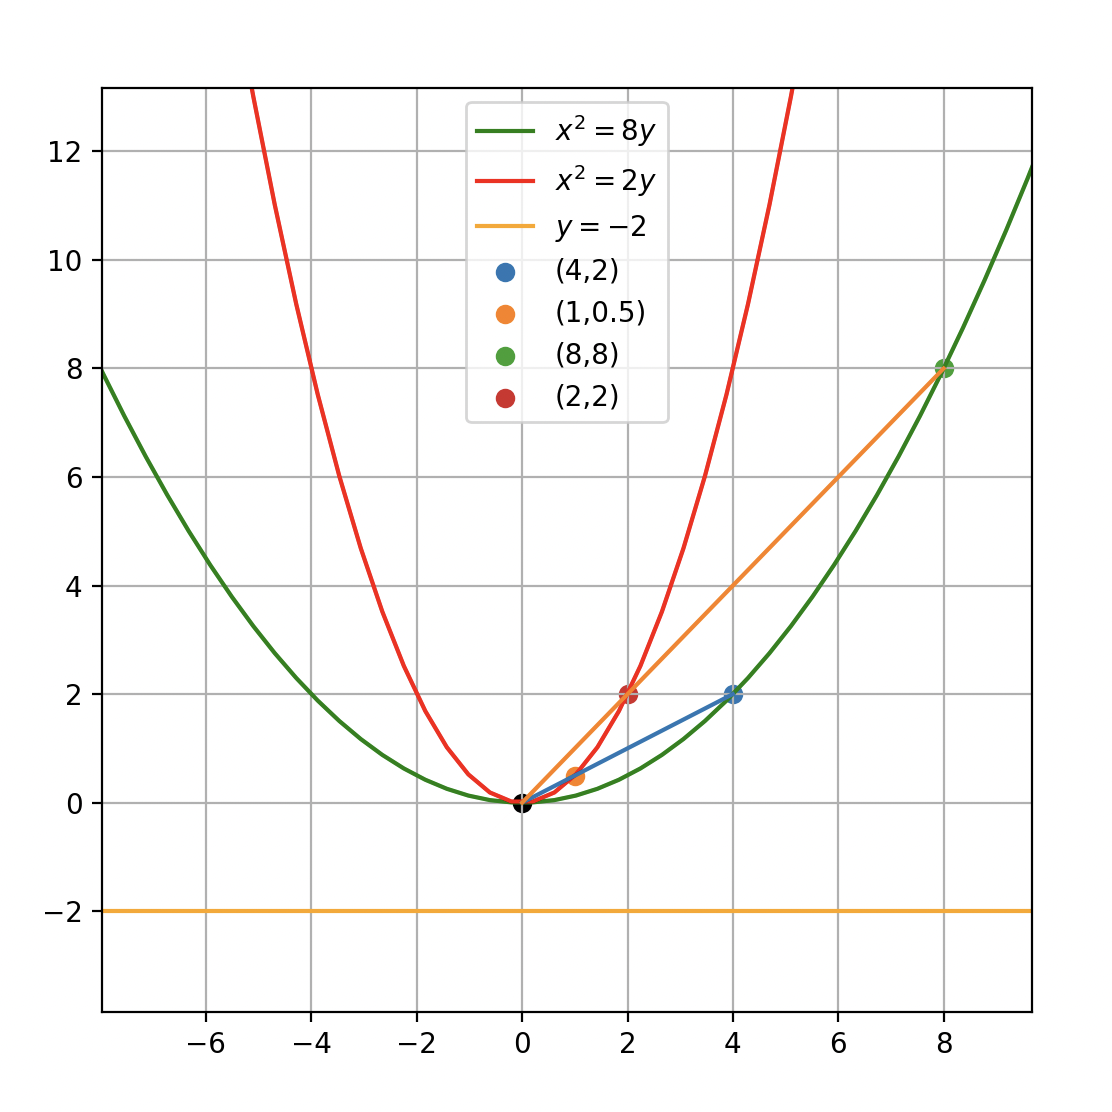
\includegraphics[width=0.9\columnwidth]{Figs/847.png}
    \caption{Plot}
    \label{fig:placeholder}
\end{figure}


\end{document}